\documentclass[11pt]{article}

\usepackage[margin=1in]{geometry}
\usepackage[utf8]{inputenc}
\usepackage[T1]{fontenc}
\usepackage{lmodern}
\usepackage{amsmath}
\usepackage{amssymb}
\usepackage{booktabs}
\usepackage{graphicx}
\usepackage{array}
\usepackage{xcolor}
\usepackage{hyperref}
\usepackage{float}

\graphicspath{{report_fig/}}

\hypersetup{
    colorlinks=true,
    linkcolor=teal!70!black,
    urlcolor=teal!70!black,
    citecolor=teal!70!black,
}

\setlength{\emergencystretch}{3em}

\title{\textbf{Smart Grocer:} A Web-Scraping and Statistical Analysis\\
of Cross-Retailer Grocery Pricing}
\author{Ellie Burton \\ Capstone in Data Science}
\date{Spring 2026}

\begin{document}

\maketitle

\begin{abstract}
\noindent
Grocery prices vary by retailer and location, but consumers, and college
students in particular, lack a unified way to compare baskets without
manually visiting each store's website. \textit{Smart Grocer} is a
locally run Python application that automates this comparison: a
Selenium and HTTP-based scraping engine collects real-time prices from
\textbf{Aldi}, \textbf{Publix}, and \textbf{Walmart}; an enrichment
pipeline standardizes units and brands; and a Streamlit interface
delivers a ``best basket'' recommendation. Over a 37-day window the
system was scheduled to capture a fixed 12-item basket daily, producing
a longitudinal panel of 1{,}332 observations. A Randomized Complete
Block Design treated items as blocks and retailers as treatments. The
Friedman test on item-level mean prices did \textit{not} detect a
significant overall retailer effect ($\chi^2_F = 5.17$, $p = 0.0755$),
but per-category Friedman tests were highly significant in every
category, and a multi-store optimization strategy reduced the average
daily cost from \$32.95 (best single store, Walmart) to \$26.35, a mean
saving of \$6.59 per day. A day-of-week effect was \textit{not}
detected. The report also discusses the practical limitations imposed
by retailer bot defences, including the decision to abandon zip-code
specific store selection in favor of IP geolocation.
\end{abstract}

\section{Introduction}

Weekly grocery shopping is one of the most consistent recurring
expenses for households, and especially for college students operating
on tight budgets. Yet finding the cheapest combination of goods across
nearby retailers is largely manual: a shopper has to visit each store's
website, enter their zip code, search for each item, and mentally
aggregate prices. Differences in package sizes, store brands, and
promotional labels make even simple comparisons surprisingly difficult.

Smart Grocer addresses this problem with two services that share the
same scraping engine. The first is an interactive Streamlit web app
that takes a grocery list and zip code and returns a ``cheapest
basket'' recommendation across Aldi, Publix, and Walmart. The second is
a daily-scheduled job that scrapes a fixed 12-item basket to build a
time series suitable for formal statistical inference. The longitudinal
dataset enables five research questions originally outlined in the
project proposal: controlling for product-specific variance, do mean
prices differ between retailers; is the retailer effect consistent
across categories; which items and which retailer exhibit the highest
price volatility; is there a day-of-week effect on basket cost; and
can the consumer save money by splitting the basket across multiple
stores rather than shopping at a single retailer?

\section{Methods: Data Collection}

The collection layer (\texttt{main.py}) is a Python pipeline that
launches three retailer-specific scrapers concurrently. Aldi
(\texttt{scrapers/aldi.py}) and Publix (\texttt{scrapers/publix.py})
both use Selenium to drive the Instacart-powered storefronts now
shared by both retailers, while Walmart (\texttt{scrapers/walmart.py})
is fetched via plain HTTP using realistic Chrome-derived
\texttt{User-Agent} headers and parsed with \texttt{BeautifulSoup},
which avoids the most aggressive anti-bot challenges entirely. To keep
Selenium and \texttt{User-Agent} strings in sync with the local
browser, \texttt{scrapers/utils.py} detects the installed Chrome
version and pins the driver accordingly. Each scraper returns up to
five matched product cards per term, after a token-based keyword
filter rejects irrelevant matches. Longitudinal collection is driven
by \texttt{run\_daily\_basket.py}, which loads the fixed 12-item list
from \texttt{config.py} (Whole Milk, Large Eggs, Salted Butter,
Bananas, Gala Apples, Iceberg Lettuce, Ground Beef 80/20, Chicken
Breast, White Bread, Spaghetti Pasta, Tomato Sauce, Dish Soap),
appends \emph{all} surviving matches (typically up to five rows per
(date, store, item) cell) to \texttt{data/daily\_basket.csv} with a
fixed canonical column order, and is scheduled via Windows Task
Scheduler to run once per day. The raw longitudinal file therefore
contains roughly $5 \times 12 \times 3 \times 37 \approx 6{,}500$
candidate rows; the analysis panel is a downstream selection from
this raw file (Section~\ref{sec:enrich}).

\subsection{Enrichment pipeline}\label{sec:enrich}

Raw scraper output is messy: prices appear as strings such as
\texttt{"Current price: \$3.99"} or even \texttt{"\$448current price
\$4.48"}, and unit sizes range from \texttt{"1 gal"} through
\texttt{"avg.\ 1.33 lb/package (\$5.59/lb)"}. The enrichment module
(\texttt{lib/enrich.py}) standardizes every row before it reaches the
analysis layer. Price parsing extracts a numeric \texttt{clean\_price}
using regular expressions that prefer the ``current price'' decimal
pattern and reject values above \$500 as artefacts. Unit normalization
(\texttt{scrapers/units.py}) converts gallons to 128 oz, pounds to 16
oz, and dozens to 12 count, with dedicated rules for packs, sticks,
bottles, and loaves; ambiguous strings set \texttt{unit\_uncertain},
and price per unit is then $\text{clean\_price} /
\text{normalized\_qty}$. Each row is also tagged with a brand type
(\texttt{Private} for known store-brand prefixes such as
\textit{Great Value} or \textit{Friendly Farms},
\texttt{National} otherwise), a category (Dairy, Produce, Meat,
Pantry, or Household), and a token-overlap match score with synonym
expansion; rows whose score falls below 0.5 are flagged
\texttt{name\_match\_uncertain} and dropped from analysis.

A final row-selection step collapses each (date, store, item) cell to
a single representative row by taking the surviving candidate with
the lowest \texttt{price\_per\_unit}. This mirrors the behavior of
the Streamlit ``cheapest basket'' recommender, which always surfaces
the best per-unit deal at each store, and ensures the longitudinal
panel describes the price a rational shopper would actually pay
rather than a noisy mixture of package sizes (e.g.\ a half-gallon
versus a gallon of milk on the same shelf). The selection rule is
applied after, not before, the keyword and \texttt{name\_match}
filters so that an irrelevant low-priced match (such as a pecan-milk
result for a ``whole milk'' query) cannot drive the choice.

\section{Data}

The analysis dataset is \texttt{data/daily\_basket\_cleaned.csv}: 37
consecutive observation dates between February 3 and March 11, 2026.
The raw collection file (\texttt{data/daily\_basket.csv}) holds the
top-five product matches per (date, store, item) cell. Applying the
cheapest-per-unit selection rule from Section~\ref{sec:enrich}
collapses each cell to a single row, producing a fully populated
$12 \times 3$ basket on every date and \textbf{1{,}332 rows} in the
analysis panel (12 items $\times$ 3 stores $\times$ 37 dates), with
no dates dropped. Of those rows, 74 were originally flagged
\texttt{unit\_uncertain}, all from Publix on Whole Milk and Iceberg
Lettuce where the scraper failed to capture a \texttt{unit\_size}.
Dropping them would have left Publix with an 11-item basket on those
days and artificially deflated its basket cost, so we imputed the
canonical sizes used by the other retailers (Whole Milk to 128 oz,
Iceberg Lettuce to 1 count); the \texttt{unit\_uncertain} count is 0
after imputation.

Mean daily basket cost was \$33.16 at Aldi, \$38.38 at Publix, and
\$32.95 at Walmart (Table~\ref{tab:basket-summary},
Figure~\ref{fig:mean-basket}). Aldi and Walmart are effectively tied,
while Publix runs roughly \$5.43 per day more than Walmart and \$5.22
more than Aldi, with roughly twice their day-to-day standard
deviation.

\begin{table}[H]
\centering
\caption{Daily basket cost summary (\$), $n = 37$ dates per store.}
\label{tab:basket-summary}
\begin{tabular}{@{}lrrrrr@{}}
\toprule
\textbf{Store} & \textbf{Mean} & \textbf{SD} & \textbf{Min} & \textbf{Max} & \textbf{\$/item} \\
\midrule
Aldi    & 33.16 & 0.34 & 32.32 & 33.64 & 2.76 \\
Publix  & 38.38 & 0.65 & 37.66 & 40.06 & 3.20 \\
Walmart & 32.95 & 0.47 & 31.83 & 33.43 & 2.75 \\
\bottomrule
\end{tabular}
\end{table}

\begin{figure}[H]
\centering
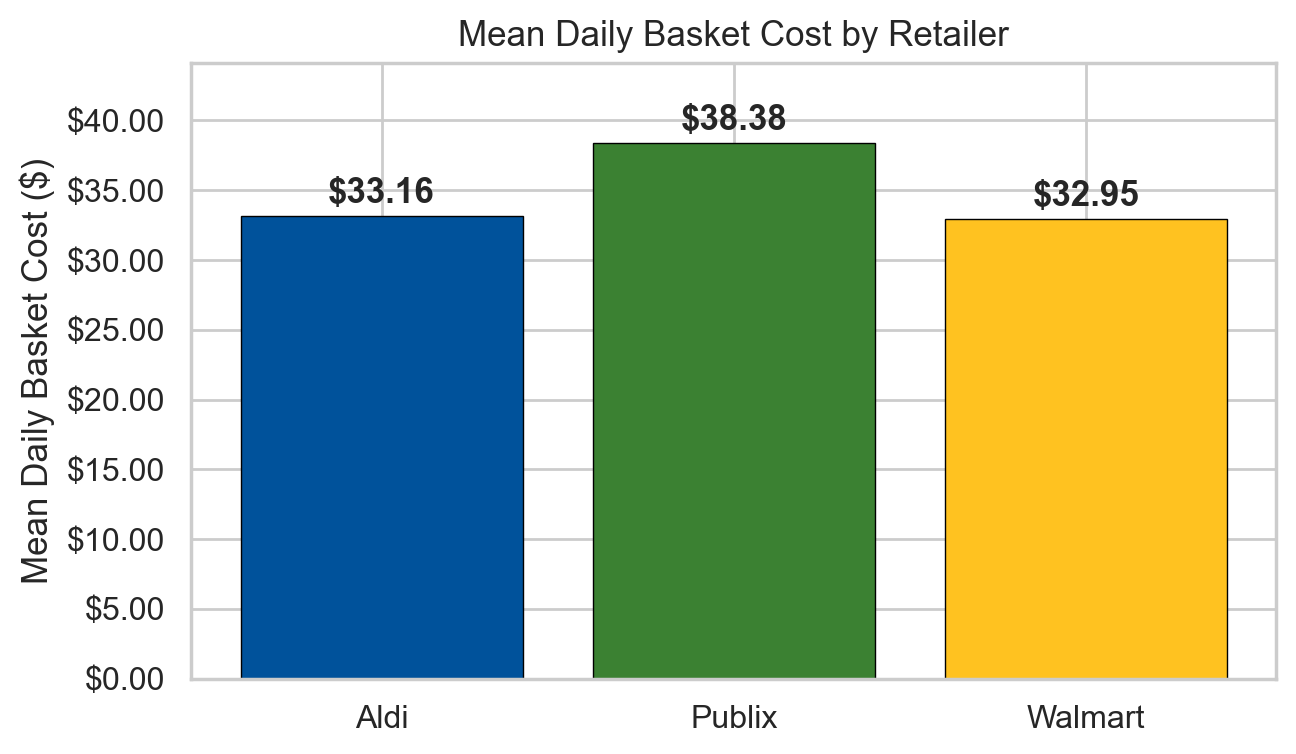
\includegraphics[width=0.62\linewidth]{02_mean_basket_bar.png}
\caption{Mean daily basket cost by retailer over the 37-day window.
Aldi and Walmart are effectively tied; Publix sits roughly \$5 higher
per day.}
\label{fig:mean-basket}
\end{figure}

\section{Analysis}

\subsection{RCBD with item blocking}\label{sec:rcbd}

Item identity is the dominant source of nuisance variance in any
grocery panel: chicken breast costs roughly 30 times more than
bananas. To isolate the retailer effect, items are treated as blocks
and retailers as treatments in a Randomized Complete Block Design.
For each (item, store) cell we average across the 37 dates, producing
a $12 \times 3$ matrix. The Friedman test then asks whether the
within-item store rankings are consistent enough across items to
conclude that stores differ systematically.

Two assumption checks were performed first. The Shapiro-Wilk test on
the RCBD residuals gives $W = 0.883$, $p = 0.0012$, so normality is
rejected (heavy tails are driven by a few items with large inter-store
gaps such as Chicken Breast and Tomato Sauce). Levene's test on the
store columns is comfortably non-significant ($F = 0.144$,
$p = 0.866$), so unequal variance is not a concern. With normality
violated on a small ($n = 36$) residual sample, the analysis pivots to
the non-parametric Friedman Rank Sum Test, which yields
\[
\chi^2_F = 5.17, \quad p = 0.0755, \quad k = 3 \text{ stores}, \quad b = 12 \text{ items}.
\]
At $\alpha = 0.05$ the omnibus test fails to reject the null of equal
store ranks. Although Publix is visibly more expensive in aggregate
(Figure~\ref{fig:mean-basket}), that gap is driven by a handful of
items; when each of the 12 items casts an equal vote, the rankings
are inconsistent enough that the omnibus test is not significant.
Pairwise Wilcoxon signed-rank tests on the 12 matched item means
(Table~\ref{tab:posthoc}) confirm this result: no pair differs
significantly. Aldi and Walmart are nearly tied on basket cost, while
Publix runs about \$5 per day higher.

\begin{table}[H]
\centering
\caption{Post-hoc pairwise Wilcoxon signed-rank tests on item mean
prices. ``Wins'' counts items for which the first store is strictly
cheaper.}
\label{tab:posthoc}
\begin{tabular}{@{}lrrrrr@{}}
\toprule
\textbf{Comparison} & \textbf{Mean diff (\$)} & \textbf{A wins} & \textbf{B wins} & \textbf{W} & \textbf{p} \\
\midrule
Aldi vs.\ Publix    & $-0.44$           & 8 & 4 & 27 & 0.380 \\
Aldi vs.\ Walmart   & $\phantom{-}0.02$ & 3 & 9 & 21 & 0.176 \\
Publix vs.\ Walmart & $\phantom{-}0.45$ & 3 & 9 & 17 & 0.092 \\
\bottomrule
\end{tabular}
\end{table}

\subsection{Category-level Friedman tests}

The omnibus result hides clear category effects. Re-running Friedman
\emph{within} each of the five categories, using daily total category
cost as the response across the 37 dates, yields a strongly
significant result in every category (Table~\ref{tab:cat}). The
retailer effect is real but \textit{category-dependent}: store
rankings are consistent within categories, but the cheapest store is
not the same in every category, so the within-item ranks cancel out
in the omnibus test. Figure~\ref{fig:interaction} makes this visible:
the curves are far from parallel, with Meat exhibiting the largest
spread between cheapest and most expensive store, and Aldi tending to
win Dairy and Meat while Walmart tends to win Produce and Pantry.

\begin{table}[H]
\centering
\caption{Friedman tests on daily category cost (per category).}
\label{tab:cat}
\begin{tabular}{@{}lrrrl@{}}
\toprule
\textbf{Category} & \textbf{n (dates)} & \textbf{$\chi^2$} & \textbf{p} & \textbf{Significant} \\
\midrule
Dairy     & 37 & 68.49 & $<0.0001$ & $\checkmark$ \\
Household & 37 & 74.00 & $<0.0001$ & $\checkmark$ \\
Meat      & 37 & 74.00 & $<0.0001$ & $\checkmark$ \\
Pantry    & 37 & 74.00 & $<0.0001$ & $\checkmark$ \\
Produce   & 37 & 56.16 & $<0.0001$ & $\checkmark$ \\
\bottomrule
\end{tabular}
\end{table}

\begin{figure}[H]
\centering
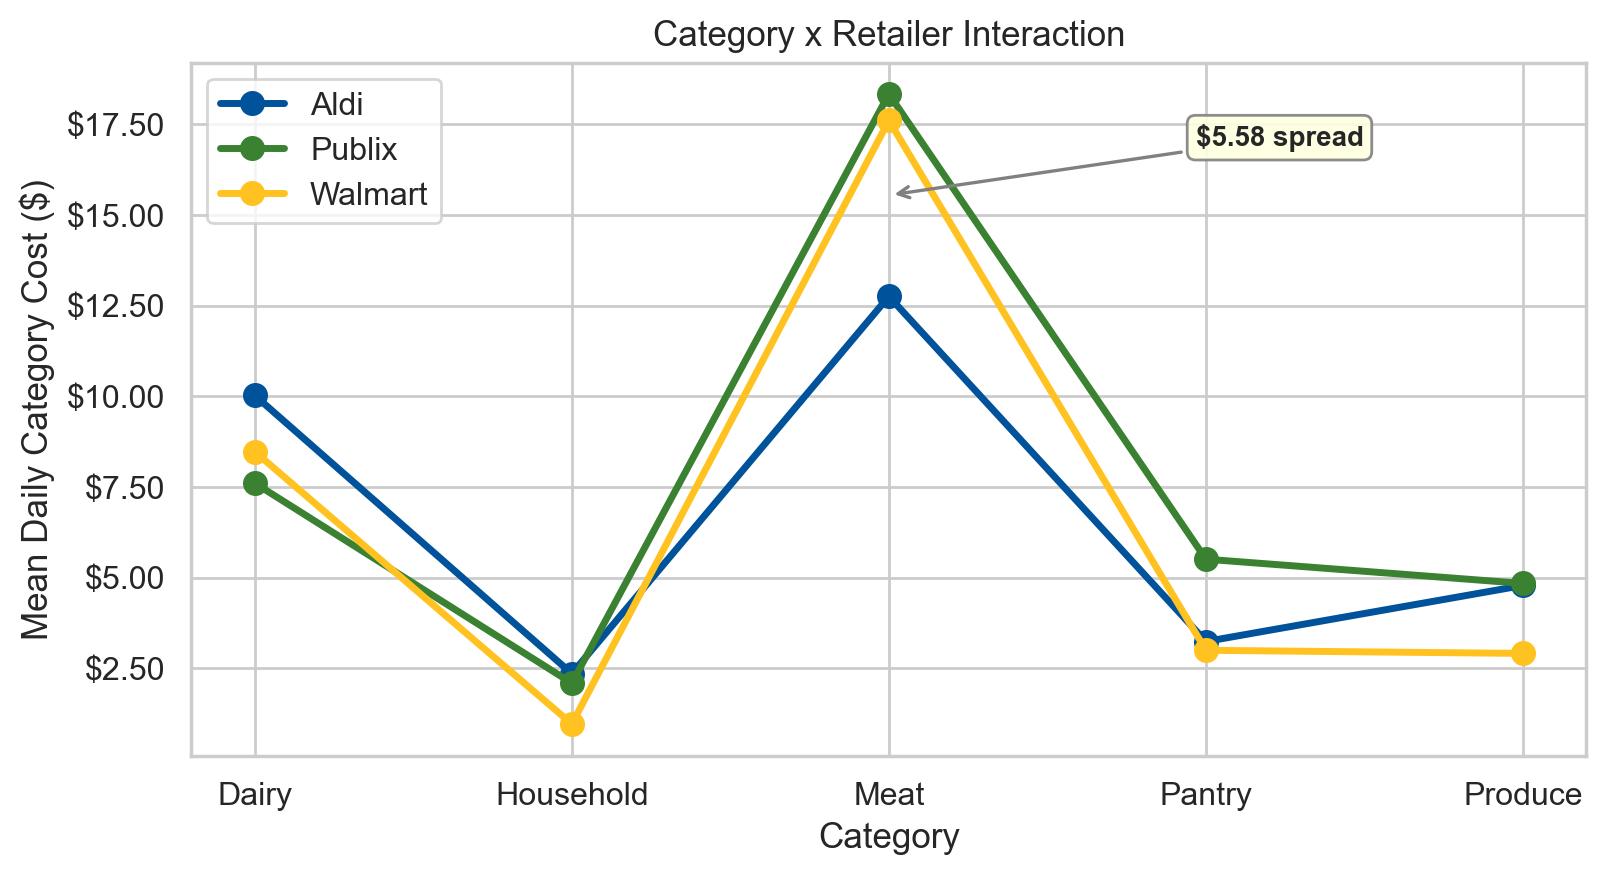
\includegraphics[width=0.72\linewidth]{05_category_interaction.png}
\caption{Category $\times$ Retailer interaction: mean daily category
cost. Lines are far from parallel, indicating that the retailer's
price advantage depends on the category. Meat shows the largest
spread between cheapest and most expensive store.}
\label{fig:interaction}
\end{figure}

\subsection{Volatility, day-of-week, and multi-store optimization}

Because items have very different price levels (bananas at \$0.16
versus chicken breast at over \$10), volatility is reported as the
coefficient of variation $\text{CV} = \sigma/\mu$. Bananas is the
most volatile item with a mean CV of approximately 13.6\%, an
artefact of weight-based pricing on naturally variable produce, while
Ground Beef 80/20 is the least volatile at roughly 0.9\%. At the
category level, Produce is the most volatile across all three
retailers and Household is the most stable
(Table~\ref{tab:cv}, Figure~\ref{fig:cv-cat}). When pooled across all
items in a store, Walmart shows the highest overall coefficient of
variation, reflecting wider product-level price spread rather than
week-to-week instability.

\begin{table}[H]
\centering
\caption{Coefficient of variation of daily category cost by retailer.}
\label{tab:cv}
\begin{tabular}{@{}lrrr@{}}
\toprule
\textbf{Category} & \textbf{Aldi} & \textbf{Publix} & \textbf{Walmart} \\
\midrule
Dairy     & 0.0154 & 0.0643 & 0.0101 \\
Household & 0.0119 & 0.0122 & 0.0261 \\
Meat      & 0.0133 & 0.0032 & 0.0238 \\
Pantry    & 0.0372 & 0.0734 & 0.0355 \\
Produce   & 0.0962 & 0.0403 & 0.0667 \\
\bottomrule
\end{tabular}
\end{table}

\begin{figure}[H]
\centering
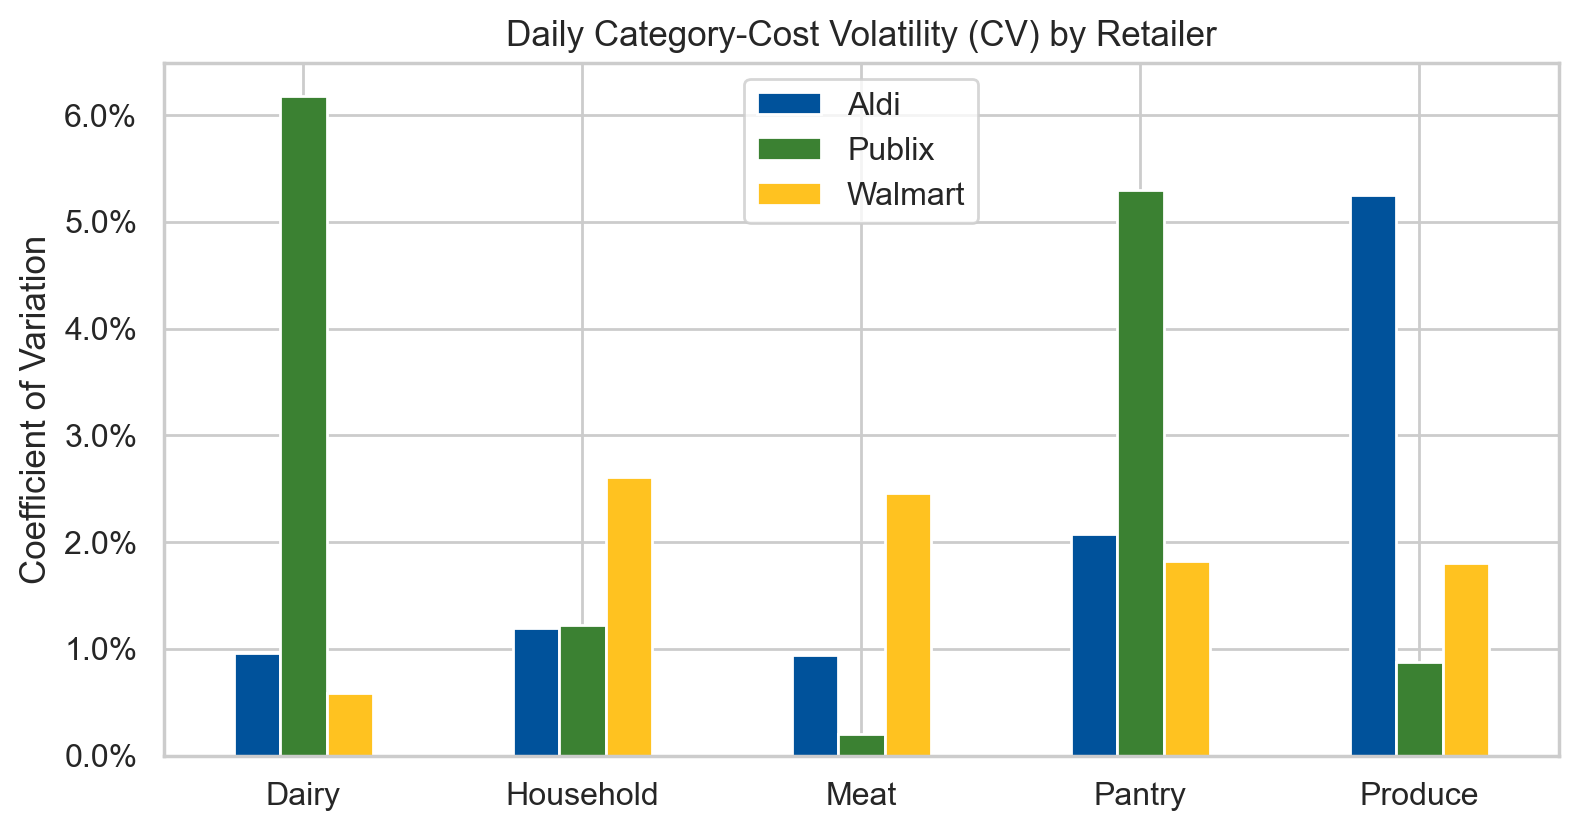
\includegraphics[width=0.62\linewidth]{07_cv_by_category.png}
\caption{Coefficient of variation of daily category cost, by retailer.
Produce is the most volatile category across all three stores;
Household is the most stable.}
\label{fig:cv-cat}
\end{figure}

The Kruskal-Wallis $H$-test on basket cost by day of week is
decisively non-significant ($H = 0.23$, $p = 0.9998$) both pooled
across stores and within each store individually (Aldi $p = 0.97$,
Publix $p = 0.98$, Walmart $p = 0.95$). The shopping-folklore claim
that ``Tuesday is cheaper'' is not supported by the data.

For each (date, item) pair the cheapest of the three stores is
selected and the savings are summed across the 12 items. The
resulting ``optimal split'' basket has a daily mean of \$26.35,
compared with a best single-store mean of \$32.95 (Walmart). The mean
additional saving from splitting the basket across stores, on top of
always shopping at the cheapest single store, is \textbf{\$6.59 per
day}, with a maximum single-day saving of \$7.12. Cherry-picking the
cheapest store per item saves roughly 20\% relative to the best
single-store strategy, and Figure~\ref{fig:cheapest} shows why: no
store dominates more than six or seven items. Walmart wins on Dish
Soap, Gala Apples, and Tomato Sauce; Aldi wins on Bananas and Chicken
Breast; Publix is rarely cheapest, with Salted Butter the most common
exception. The day-by-day gap between the best single store and the
optimal split basket is shown in Figure~\ref{fig:split}.

\begin{figure}[H]
\centering
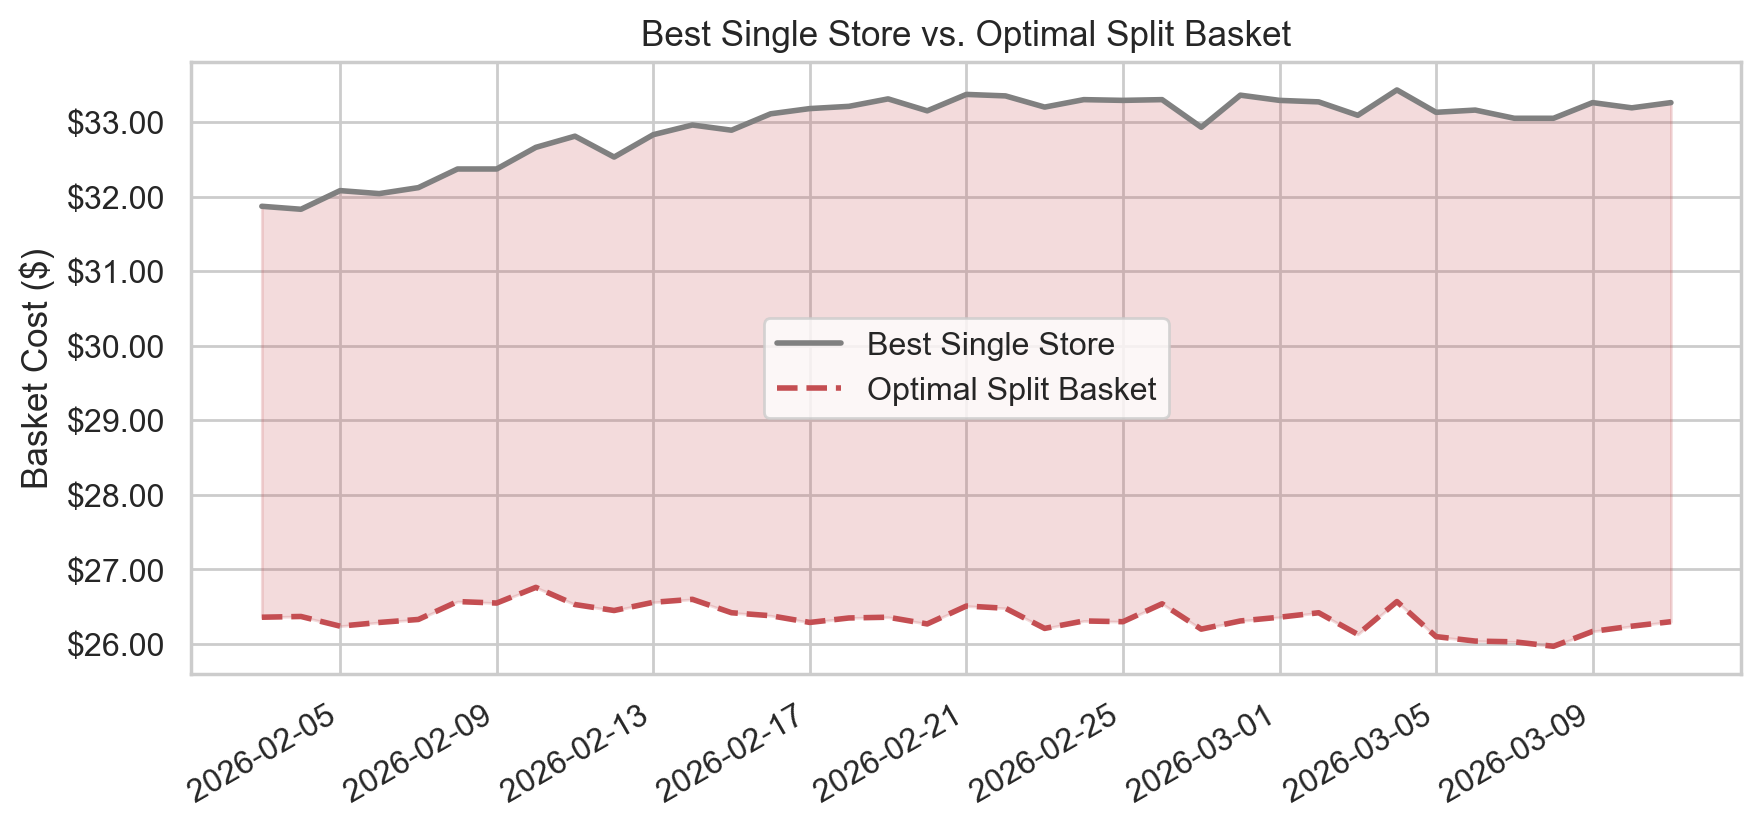
\includegraphics[width=0.78\linewidth]{10_split_vs_single.png}
\caption{Best single store vs.\ optimal split basket. The shaded band
is the daily saving available from splitting across multiple stores,
averaging \$6.59 per day.}
\label{fig:split}
\end{figure}

\begin{figure}[H]
\centering
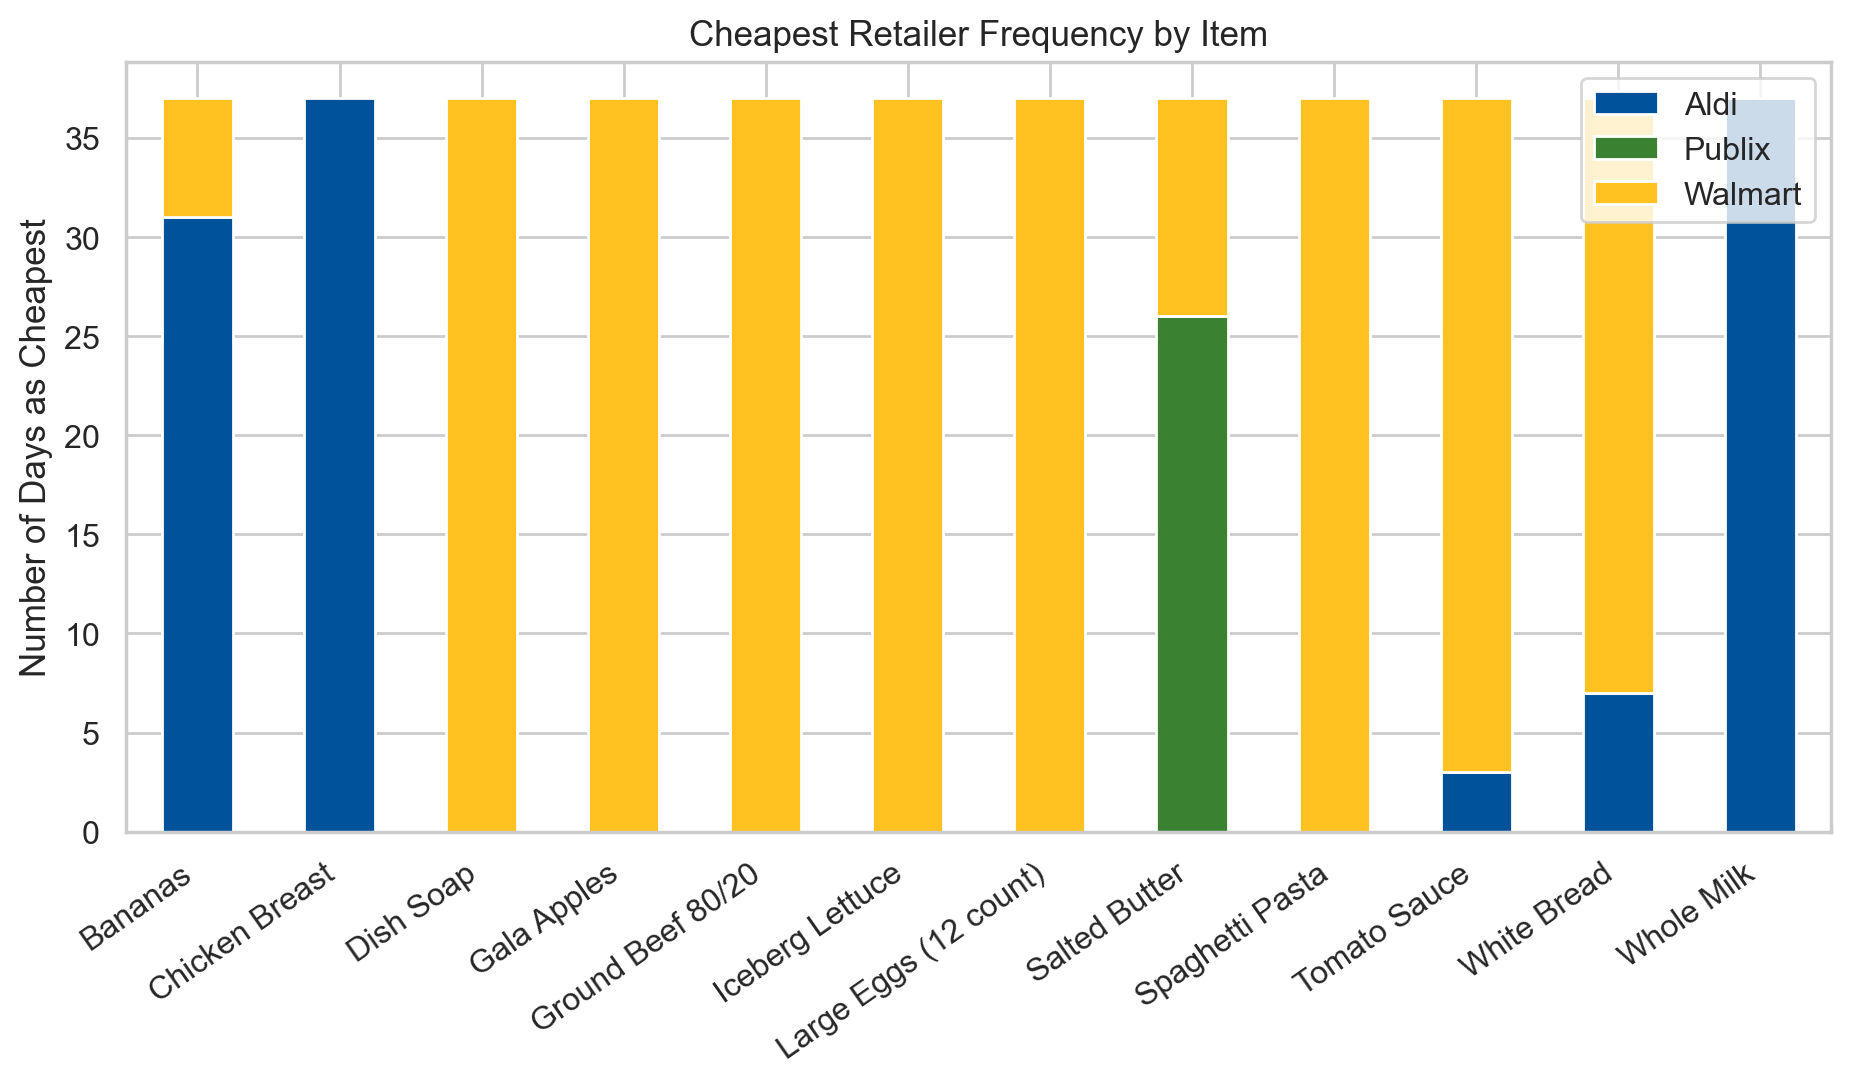
\includegraphics[width=0.85\linewidth]{11_cheapest_by_item.png}
\caption{Cheapest retailer frequency by item. No store dominates more
than six or seven of the twelve items, which is why splitting the
basket pays.}
\label{fig:cheapest}
\end{figure}

\section{Limitations}\label{sec:limitations}

\subsection{The zip-code pivot}\label{sec:zip-pivot}

The original proposal promised \textbf{location-specific pricing}: the
user would enter a zip code, the scraper would set the corresponding
store, and the returned prices would reflect that store's local
shelves. This worked for most of the semester, but mid-project changes
to the Instacart platform (which now powers both the Aldi and Publix
online stores) made automated zip-code entry unreliable enough that
we abandoned the feature and pivoted to IP-based geolocation. Walmart
(issue~\#2 in \texttt{issues.md}) hit the same wall earlier: the
store-finder modal could only be driven through Selenium, which was
reliably blocked by Walmart's PerimeterX/HUMAN bot detection, so
location selection was removed and the site's IP-based fallback was
used. Publix (issues~\#5, \#17--\#19) lives inside an Instacart portal
with frequently rotating CSS class names, and even after detailed
debugging in
\texttt{run\_publix\_\allowbreak location\_\allowbreak debug.py}
we could not obtain a stable click sequence. Aldi (issues~\#3, \#4)
was hit by a wholesale migration to the same Instacart storefront
mid-project, breaking every legacy CSS selector; the scraper was
rewritten to use the Instacart card-parsing approach used for Publix,
again without per-zip store selection. The consequence is that the
reported prices reflect a single de-facto location (the IP geolocation
of the machine running the scrapers, plus the Instacart default for
Aldi and Publix). All inferential conclusions in this report should be
read as ``relative to this implicit location''.

\subsection{Bot detection, scraper fragility, and data quality}

Several other failure modes from \texttt{issues.md} affected the data
pipeline. Walmart's ``robot or human'' interstitial occasionally fired
even with \texttt{undetected\_\allowbreak chromedriver} (issue~\#1);
the HTTP fallback now carries the primary load. Walmart scraper
exceptions were originally swallowed under a generic ``a scraper
crashed'' message (issue~\#23), so on those days no Walmart rows were
appended at all; per-store crash reporting was added in response, but
pre-existing missing days cannot be recovered. Publix result lists in
the Instacart SPA re-render mid-iteration, occasionally raising
\texttt{StaleElementReferenceException} (issue~\#24), which
index-based iteration with retry mitigates but does not eliminate.
A Chrome auto-update once pushed the local browser to a major version
that the cached ChromeDriver did not support, killing two days of
runs before version pinning was added (issue~\#22).

Data-quality issues had a more direct effect on the cleaned prices.
Early Walmart fallback parsing produced concatenated strings such as
\texttt{"\$448current price \$4.48"} (issue~\#10) from which a naive
regex would extract \$448; the ``current price'' decimal-prefix
heuristic in \texttt{lib/enrich.py} resolves this going forward but
earlier rows could in principle still contain artefacts. Generic
searches such as ``bananas'' or ``eggs'' originally returned
irrelevant results like chips or muffins (issue~\#12); token-based
keyword filtering and the \texttt{name\_match\_uncertain} flag
suppress this, and the \texttt{daily\_basket\_cleaned.csv} variant
was used for analysis to ensure these fixes are applied uniformly.
Bananas and ground beef are sold per pound but listed with both
per-package and per-pound prices (issue~\#13); guardrails on
synthetic variability magnitude reduce, but do not eliminate, the
chance that an unusually cheap row reflects a per-pound vs.\ per-each
mismatch. The 74-row imputation of Publix Whole Milk and Iceberg
Lettuce is similarly a reasonable but non-trivial assumption that any
per-unit comparison involving these rows inherits.

\subsection{Statistical and design limitations}

The 37-day observation window is enough to detect persistent ranking
effects but not seasonal patterns, sale cycles, or holiday spikes,
and the day-of-week null result should be read in that light. Single
zip collection (Section~\ref{sec:zip-pivot}) precludes any
cross-region generalization. The RCBD design has $b = 12$ blocks and
$k = 3$ treatments, which gives limited power: the omnibus Friedman
result ($p = 0.076$) is suggestive but not significant, and a longer
window or wider basket would tighten the test. Independence of
basket items, which the Friedman test assumes, is mildly violated by
retailer-wide shocks such as inflation or category-level discounts.
None of the analyses here support a causal claim: we describe
observed rankings and means but cannot speak to \textit{why} a given
retailer is cheapest in a given category. The slide deck also notes
that vague search terms (e.g.\ ``lettuce'' returning a head at one
store and a bagged shredded product at another) and the assumption of
zero travel cost in the multi-store optimization are real
limitations: a \$6.59 daily saving may not be worth a 45-minute round
trip and \$3 in gas. A fuel-and-time-aware ``cost of detour''
variable, anticipated as a possible extension in the original
proposal, would convert the savings figure into a true break-even
threshold.

\section{Conclusion}

Smart Grocer demonstrates an end-to-end pipeline (live web scraping,
schema enrichment, longitudinal storage, and formal statistical
inference) applied to a question every shopper has informally asked:
\textit{which grocery store is actually cheapest?} The answer that
emerges from 37 days of data is more nuanced than the project's
proposal anticipated. There is no statistically significant overall
winner when each of 12 items votes equally
($\chi^2_F = 5.17$, $p = 0.0755$); within each category the ranking
of stores is extremely stable, but the cheapest store changes across
categories, with Aldi and Walmart trading the top spot depending on
basket contents. Day-of-week pricing folklore is not supported by the
data, and a consumer willing to make two stops can save approximately
\$6.59 per day, or about 20\%, relative to the best single store,
which is the largest practical effect in the study. The project also
illustrates the cost of building a real scraping system: bot defences
forced the abandonment of zip-code specific pricing, occasional
silent failures cost partial days of data, and careful enrichment is
required to turn vendor-formatted strings into analyzable numbers.
Future extensions, including multi-zip collection, a longer
observation window, stricter per-product search definitions, and the
fuel-and-time-aware ``best route'' optimization originally proposed,
all become straightforward once the longitudinal panel is large
enough to support them.

\end{document}
